\documentclass[aspectratio=169]{beamer}
% Use the metropolis theme
\usetheme{metropolis}

% booktabs for better tables
\usepackage{booktabs}
% add the logo (must be in the same directory as this file, or somewhere in your path where tex can find it)
\usetikzlibrary{positioning}
\titlegraphic{
  \begin{tikzpicture}[overlay, remember picture]
    \node[at=(current page.south east), anchor=south east] {%
      
\includegraphics[height=1.75cm]{PRIMARY_A_Vertical_Housed_RGB}
      \includegraphics[height=1.75cm]{CEBRALogo-01}
    };
  \end{tikzpicture}
}

% For twitter handle
\usepackage{fontawesome}

% Title goes here
\title{Risk Factors for Fouling Biomass: Evidence from Small Vessels in Australia}
\date{\today}
\author[Steve Lane]{Stephen E.\ Lane, \faTwitter\small{stephenelane}}
\institute{Centre of Excellence for Biosecurity Risk Analysis\\The University of Melbourne}

\setbeamertemplate{frame footer}{\includegraphics[height=0.5cm]{CEBRALogo-01}~\insertshortauthor~\faTwitter~\small{stephenelane}}

\begin{document}

\maketitle

{
  % Set a background slide picture, with nothing over the top
  \setbeamertemplate{background}{%
    \parbox[c][\paperheight][c]{\paperwidth}{%
      \centering\includegraphics[height=\paperheight]{biofouled.jpg}
    }
  }
  \begin{frame}[plain]
  \end{frame}
}

{
  % Set a background slide picture, with nothing over the top
  \setbeamertemplate{background}{%
    \parbox[c][\paperheight][c]{\paperwidth}{%
      \centering\includegraphics[height=\paperheight]{m-sallei-2.jpg}
    }
  }
  \begin{frame}[plain]
  \end{frame}
}

\begin{frame}
  \frametitle{Missingness (Vessels)}
  \centering
  \includegraphics[width=0.9\textwidth]{miss}
\end{frame}

\begin{frame}
  \frametitle{Missingness (Vessels)}
  \centering
  \includegraphics[width=0.9\textwidth]{miss2}
\end{frame}

\begin{frame}
  \frametitle{Missingness (Samples)}
  \centering
  \includegraphics[width=\textwidth]{obs_miss}
\end{frame}

\begin{frame}
  \frametitle{Censoring}
  \centering
  \includegraphics[width=\textwidth]{cens}
\end{frame}

\begin{frame}
  \frametitle{Distribution}
  \centering
  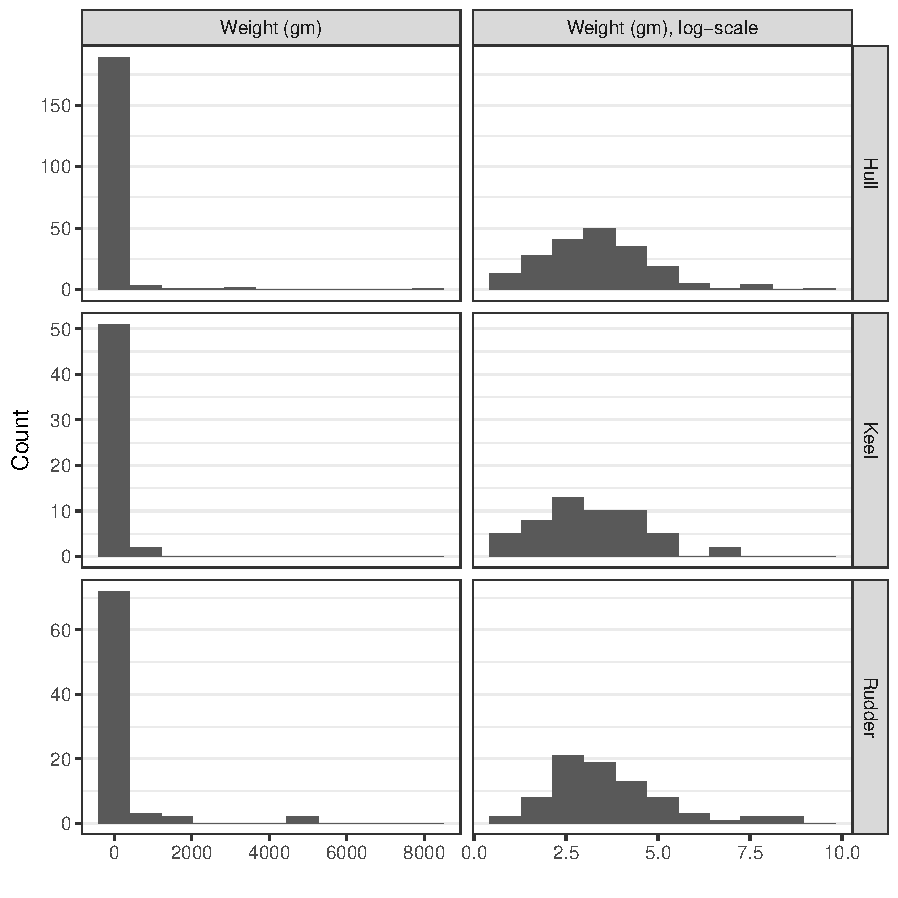
\includegraphics[height=0.8\paperheight]{../graphics/obs-hist}
\end{frame}

\begin{frame}
  \frametitle{How to Model?}
  \onslide<1->{
    \begin{enumerate}
    \item Set the samples below LOD to the `middle' value
    \item Remove those samples completely
    \item Calculate the mean wet weight biomass (for the outcome)
    \item Remove any observations with missing covariates
    \item Finally, a simple regression model
    \end{enumerate}
  }
  \onslide<2->{
    \centering {\Large \color{red}Or not!}
  }
\end{frame}

\begin{frame}
  \frametitle{Model Algorithm}
  \begin{itemize}
  \item Repeat the following a `sufficient` number of times:
    \begin{itemize}
    \item Summarise wet weight biomass by median (within vessel)
    \item Impute (via chained equations) missing vessel data
    \item Fit a censored regression (using Stan/HMC)
      \begin{align*}
        L(\theta) & = \prod_{i=1}^{n} f_{Y}(y_{i}; \theta, x)^{I(y_{i} > c)} F_{Y}(c; \theta, x)^{I(y_{i} \leq c)}
      \end{align*}
    \end{itemize}
  \item Collate chains and summarise.
  \end{itemize}
\end{frame}

% Or rather, we form a multilevel model, allow for different locations, multiple imputation, censoring. Write down the likelihood.

% \begin{frame}
%   \frametitle{Posterior Predictive Checks}
%   \centering
%   \includegraphics[height=0.8\paperheight]{../graphics/ppc-compare-m3-full}
% \end{frame}

\begin{frame}
  \frametitle{Graphical Summary}
  \centering
  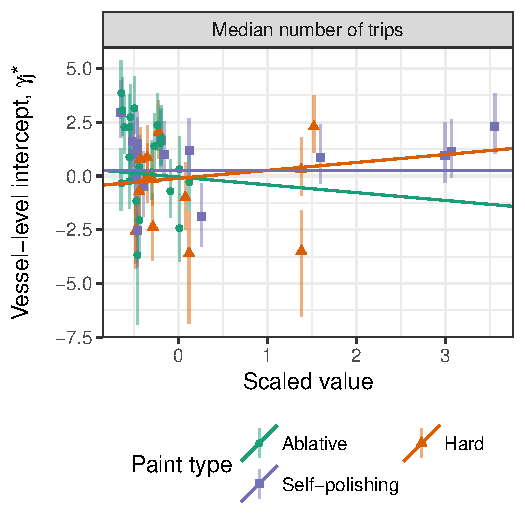
\includegraphics[height=0.8\paperheight]{../graphics/plM3paint-t}
\end{frame}

\begin{frame}
  \frametitle{Concluding Remarks}
  \begin{itemize}
  \item Relationships are largely consistent with prior expectations
  \item Limited vessels meant limited precision to estimate vessel-level effects
  \item `Simple' models inappropriate
  \item Mixture model could be a possibility (but again, limited data)
  \end{itemize}
\end{frame}

\end{document}

%%% Local Variables:
%%% mode: latex
%%% TeX-master: t
%%% End:
